\section{RM101诊断补充报告}
\label{app:rm101_diag_report}

\subsection{评估协议与样本统计}

本附录补充说明 RM101 案例的诊断协议与关键统计量。实验对象为 RM101 齿轮箱变转速、变载荷数据中的 `Dataset\_id=101`，并使用全部 `12` 个工况域进行 mixed-domain stratified split。具体而言，先按原始样本进行训练、验证、测试划分，再对每条长序列切分为 `4096` 点窗口，步长同为 `4096`，切片方式为 sliding。该设置保证了数据划分发生在窗口切分之前，从而避免窗口级数据泄漏。

本次实验的统计量如下：原始样本总数为 `240`，训练、验证、测试样本数分别为 `146/46/48`；对应窗口数分别为 `27448/8648/9024`。测试集中的 8 类标签均保持非空，其中健康样本和缺齿样本略少，其余齿轮和复合故障类别窗口数较为均衡。由于本文报告的是窗口级结果，因此表中的准确率和 Macro-F1 都反映窗口级诊断能力。

\begin{table}[!htbp]
\centering
\caption{RM101 通道物理含义说明}
\label{tab:rm101_channel_alias}
\begin{tabular}{cl}
\toprule
\textbf{通道} & \textbf{物理含义} \\
\midrule
ch1 & speed\_key\_phase（转速/键相信号） \\
ch2 & torque（转矩信号） \\
ch3 & motor\_vibration\_x \\
ch4 & motor\_vibration\_y \\
ch5 & motor\_vibration\_z \\
ch6 & gearbox\_vibration\_x \\
ch7 & gearbox\_vibration\_y \\
ch8 & gearbox\_vibration\_z \\
\bottomrule
\end{tabular}
\end{table}


\subsection{最优图谱与关键分支}

本次最优结果来自 `Gemini 2.5 Pro (simulated, all-domain mixed)` 所对应的自主诊断图谱。该图谱深度为 `5`，节点数为 `52`，边数为 `56`，终端叶子数为 `21`。与较浅图谱相比，它不仅包含 `fft` 与 `psd` 等基础谱域变换，还额外纳入了 `stft`、`patch`、`order\_track\_resample`、`tsa\_cycle\_average`、`sideband\_ratio`、`coherence` 和 `torque\_normalize` 等更具工况适应性的诊断操作，从而使整张图谱具备更强的多尺度表征能力与物理解释性。

\begin{figure}[!htbp]
\centering
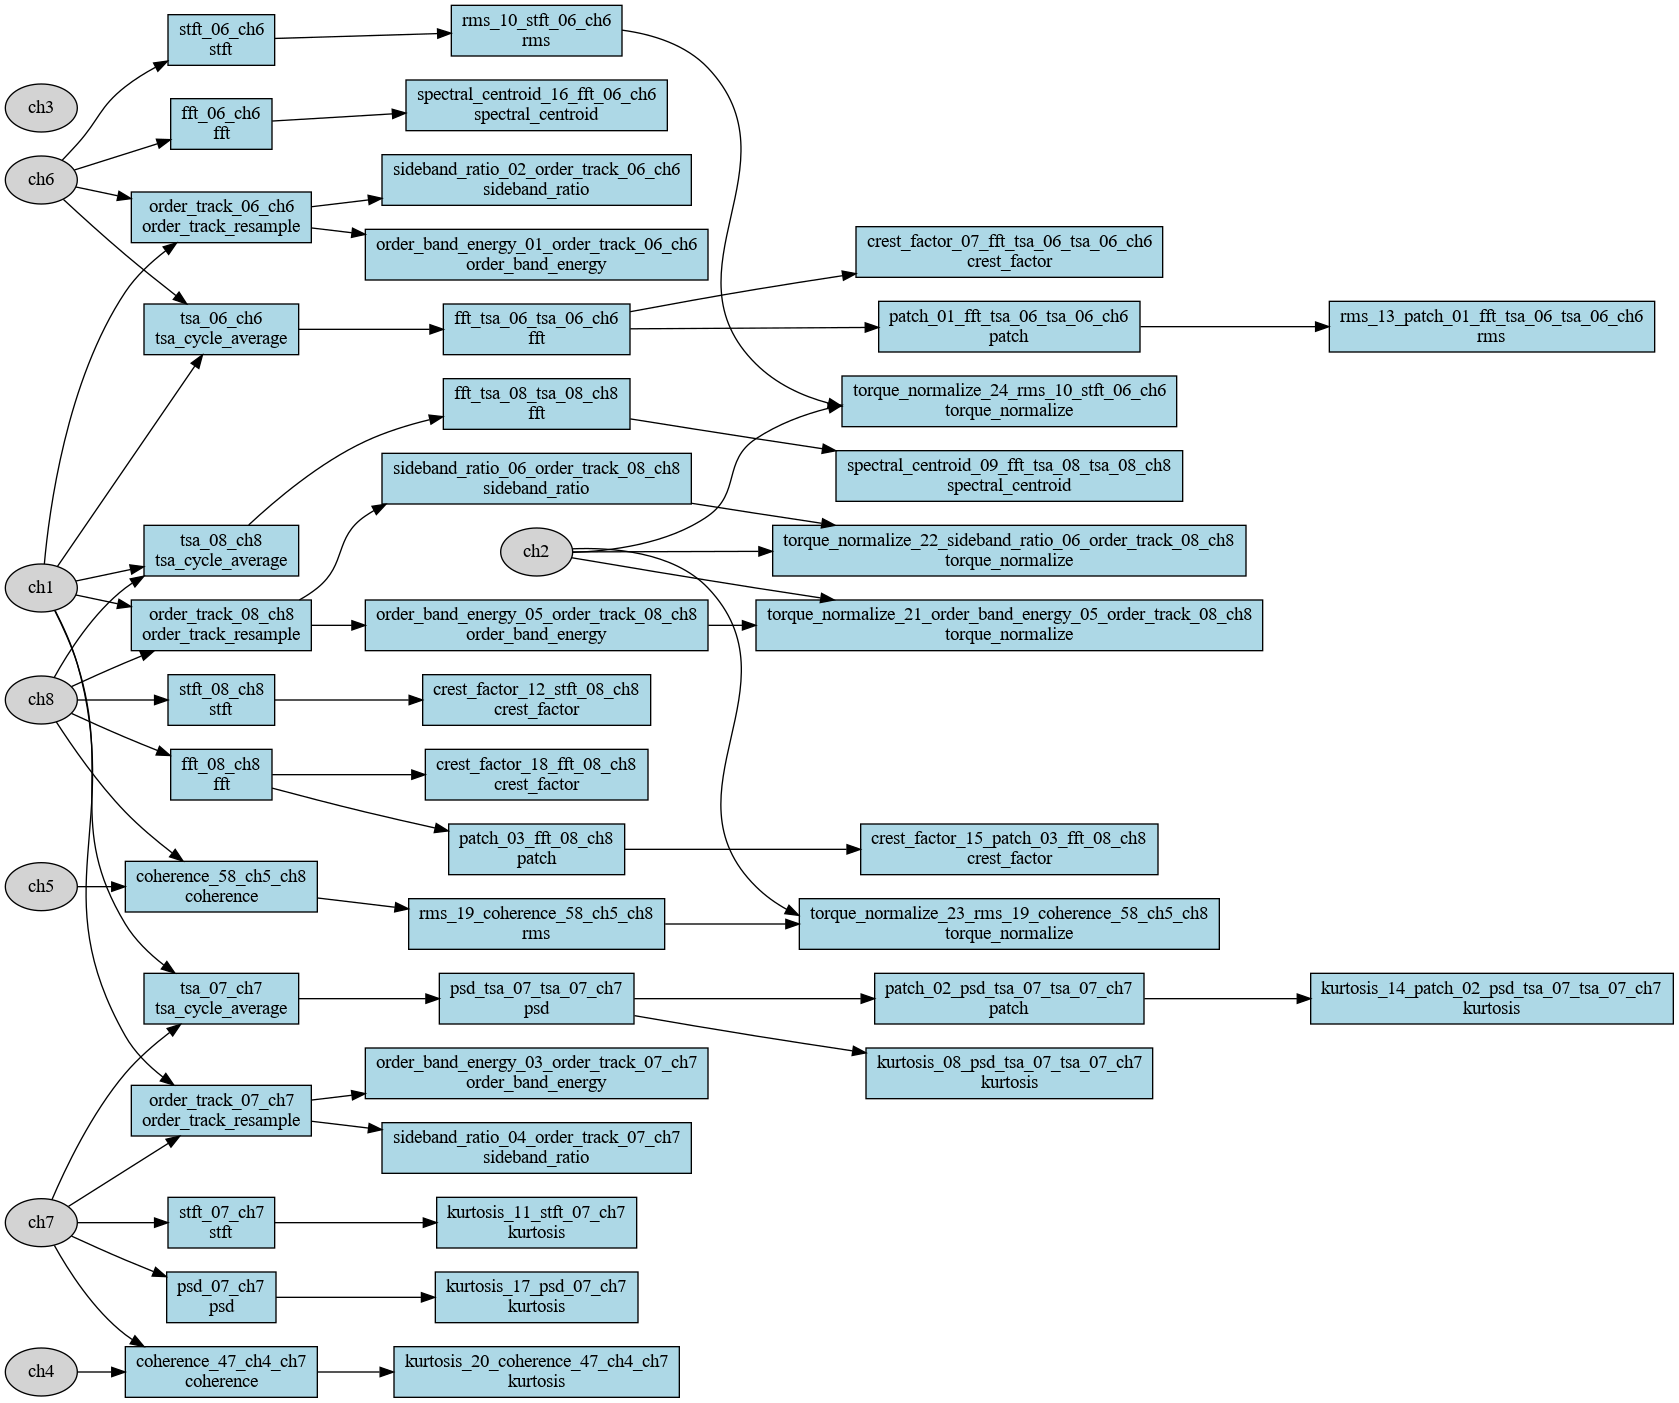
\includegraphics[width=0.95\textwidth]{figures/rm101_best_dag.png}
\caption{RM101 最优诊断图谱附图。该图在正文中用于展示整体结构，在附录中用于支撑具体诊断路径与算子组合的解释。}
\label{fig:rm101_best_dag_appendix}
\end{figure}

自动选择模块最终保留的最优叶子为 `torque\_normalize\_24\_rms\_10\_stft\_06\_ch6`，其验证集 Macro-F1 为 `0.8172`，测试集 Accuracy 和 Macro-F1 分别达到 `0.8865` 和 `0.8865`。这一结果表明，在 RM101 的复杂工况下，以齿轮箱振动通道为主、以转矩为辅助修正量的时频能量路径，最适合完成故障区分。

\subsection{候选叶子与诊断机理}

表~\ref{tab:rm101_top_leaves} 汇总了最有代表性的前 5 个候选终端叶子。可以看到，排名靠前的分支主要集中在三类机制：

\begin{itemize}
    \item `$stft \rightarrow reducer$`：强调变转速条件下的局部时频能量与尖峭度信息；
    \item `$fft/psd \rightarrow patch \rightarrow reducer$`：强调频谱局部块结构与脉冲敏感特征；
    \item `$order\_track\_resample \rightarrow order\_band\_energy$`：强调变速条件下的阶次稳定性。
\end{itemize}

\begin{table}[!htbp]
\centering
\caption{RM101 最优图谱中代表性终端叶子结果}
\label{tab:rm101_top_leaves}
\resizebox{\textwidth}{!}{%
\begin{tabular}{llcccc}
\toprule
\textbf{叶子节点} & \textbf{分支摘要} & \textbf{算法} & \textbf{特征维数} & \textbf{Val Macro-F1} & \textbf{Test Macro-F1} \\
\midrule
torque\_normalize\_24\_rms\_10\_stft\_06\_ch6 & stft $\rightarrow$ rms $\rightarrow$ torque\_normalize & MLP & 129 & \textbf{0.8172} & \textbf{0.8865} \\
crest\_factor\_15\_patch\_03\_fft\_08\_ch8 & fft $\rightarrow$ patch $\rightarrow$ crest\_factor & SVM & 64 & 0.4619 & 0.4397 \\
crest\_factor\_12\_stft\_08\_ch8 & stft $\rightarrow$ crest\_factor & SVM & 129 & 0.4551 & 0.4441 \\
kurtosis\_11\_stft\_07\_ch7 & stft $\rightarrow$ kurtosis & SVM & 129 & 0.4085 & 0.3682 \\
rms\_13\_patch\_01\_fft\_tsa\_06\_tsa\_06\_ch6 & tsa\_cycle\_average $\rightarrow$ fft $\rightarrow$ patch $\rightarrow$ rms & RandomForest & 4 & 0.3532 & 0.3267 \\
\bottomrule
\end{tabular}%
}
\end{table}


其中，最佳叶子 `$stft \rightarrow rms \rightarrow torque\_normalize$` 的优势可从三个角度理解：首先，`stft` 保留了非平稳振动在时间和频率上的联合演化；其次，`rms` 将高维时频图压缩为稳定的能量描述；最后，`torque\_normalize` 使用转矩信号对载荷波动进行补偿，使同类故障在不同负载条件下仍能保持较一致的判别边界。因此，该路径同时兼顾了复杂工况适应性和特征稳健性。

\subsection{与基线及融合结果对比}

表~\ref{tab:rm101_cross_dag_fusion} 给出了跨图谱 late fusion 的结果摘要。虽然跨图谱融合能够提升整体稳健性，并显著优于较弱的 simulated 方案，但其性能仍未超过最优单图谱。这一现象说明，在当前 all-domain mixed 设定下，最优图谱已经高度集中地编码了主要诊断信息。

\begin{table}[!htbp]
\centering
\caption{RM101 跨图谱 late fusion 结果}
\label{tab:rm101_cross_dag_fusion}
\begin{tabular}{lcc}
\toprule
\textbf{方法} & \textbf{Test Accuracy} & \textbf{Test Macro-F1} \\
\midrule
Cross-DAG Late Fusion（weighted vote） & 0.8241 & 0.8299 \\
\bottomrule
\end{tabular}
\end{table}


与真实基线比较时，需要明确区分两种结果口径：`BigModel / GLM-4.7-FlashX` 是真实运行得到的基线，而 `Gemini 2.0/2.5 Flash/2.5 Pro` 均为 simulated planner variants，代表不同复杂度的自主规划图谱梯度，而非在线 API 性能对照。即便如此，这组 simulated 梯度仍能清晰展示图谱复杂度提升所带来的诊断收益：轻量谱域图谱表现最弱，而包含时频、阶次、同步平均、跨通道关系与载荷归一化的高复杂度图谱表现最好。

\subsection{工程建议}

从工程实现与后续研究的角度看，建议优先补充以下几类能力：

\begin{itemize}
    \item 样本级诊断汇总：在窗口级结果之外，再给出原始长样本级的投票或概率平均结果；
    \item 混淆矩阵与类别级分析：明确哪些故障最容易互相混淆；
    \item 工具层物理约束：把速度、转矩与振动之间的合法连接关系写成程序规则，避免物理意义不合理的图谱分支；
    \item 概率校准：为 `SVM`、`RandomForest`、`ExtraTrees` 等模型增加校准步骤，以提高加权集成的稳定性；
    \item 跨工况泛化协议：在 mixed-domain 主结果之外，再补充 leave-one-domain-out 或 grouped-kfold 的泛化结果；
    \item DAG 模板外置：将 simulated planner 的图谱模板转成可编辑的 `yaml/json` 描述，便于诊断专家直接参与图谱修订。
\end{itemize}

综合而言，本附录支持正文中的主要结论：RM101 这类变转速齿轮箱诊断问题，需要把时频分析、工况归一化和物理约束图谱联合起来考虑；只有这样，系统才能在保持诊断可解释性的同时获得较高的测试集性能。
